%  -----------------------------------------------------------------------------
%  Author         : Bimalka Piyaruwan Thalagala
%  GitHub         : https://github.com/bimalka98
%  Date Created   : 01.09.2020
%  Last Modified  : 01.03.2020
%  -----------------------------------------------------------------------------

\documentclass[a4paper,10pt]{article}%,twocolumn
\input{settings/packages}
%% page settings
\usepackage[top=10mm, bottom=15mm,left=10mm,right=10mm]{geometry}  
 % needed for page border settings
\parindent=0mm % for space of first line of new text block

\sloppy % for writing with hyphenless justification (tries to)
\hyphenation{} % use hyphenation of tolerance parametershttp://www.jr-x.de/publikationen/latex/tipps/zeilenumbruch.html
\hyphenpenalty=10000
\exhyphenpenalty=10000
\usepackage{fancyhdr} % needed for head and foot options
\input{settings/jupyter}


\begin{document}
\begin{titlepage}
\center % Center everything on the page

%-------------------------------------------------------------------------------------
%	HEADING SECTIONS
%------------------------------------------------------------------------------------
\textbf{\large Department of Electronic and Telecommunication Engineering}\\[0.5cm]
\textbf{\Large University of Moratuwa, Sri Lanka}\\[1cm]
\textbf{\large EN2550 - Fundamentals of Image Processing and Machine Vision}\\[2cm]
\includegraphics[width=0.3\textwidth]{figures/uomlogo}\\[2cm]

	
%-------------------------------------------------------------------------------------
%	TITLE SECTION
%------------------------------------------------------------------------------------
\textbf{\Huge Assignment 01}



%----------------------------------------------------------------------------------------
%	MEMBERS SECTION
%----------------------------------------------------------------------------------------

\vfill

\textbf{\large Submitted by}\\[0.5cm]

{\large Thalagala B.P.}	\hspace{5mm} {\large 180631J }\\[1cm]

%----------------------------------------------------------------------------------------
%	DATE SECTION
%----------------------------------------------------------------------------------------

\textbf{\large Submitted on}\\[0.5cm]
\textbf{\Large \today} % Date, change the \today to a set date if you want to be precise

%----------------------------------------------------------------------------------------

 % Fill the rest of the page with whitespace

\end{titlepage}
\tableofcontents

\begin{center}
	\textbf{\textit{* PDF is clickable}}\\
\end{center}


Without the title page and the content table page there are only 6 pages in this Assignments. Only the important parts of the codes are given here due to page limitation. Complete executable code can be found at \url{https://github.com/bimalka98/Computer-Vision-and-Image-Processing/blob/main/EN2550Assignments/A1/180631J_a01.ipynb}


\pagebreak
\section{Part 1: Basic Operations}
\subsection{Histogram computation and Histogram equalization}
Histogram of an image represents the intensity distribution(\textit{intensity vs number of pixels}) over the intensities[0, 255]. Histogram equalization makes uneven histograms more or less flat. Figure (b) depicts the uneven histogram  of the original image. There, most of the red pixels are in the right region(\textit{biased to the right}) which makes the original image looks more reddish than natural. Through histogram equalization as depicted in the figure (d) the distribution can be made more uniform and it has given the image a more natural look.
\begin{figure}[!h]
	\centering
	\subfigure[Original Image]
	{ \includegraphics[scale=0.2]{figures/img0}
		
	}
	\subfigure[Hist: of the Original Image]
	{ 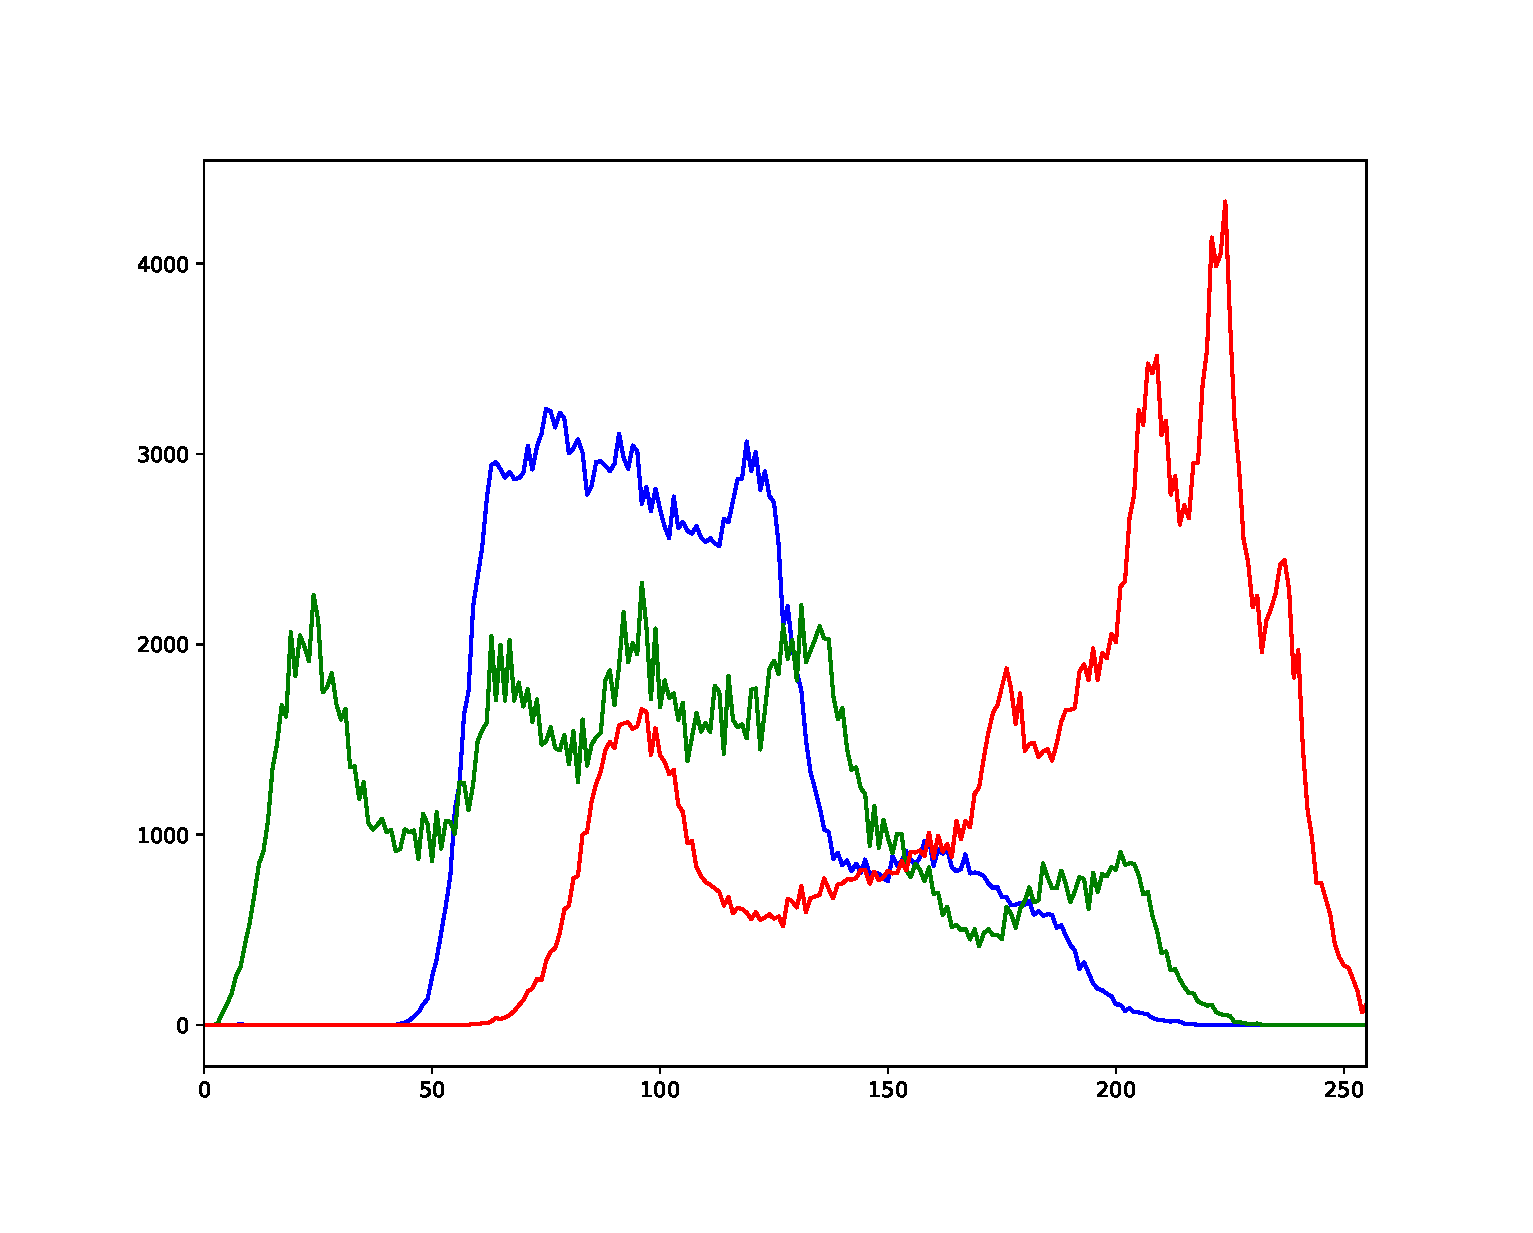
\includegraphics[scale=0.2]{figures/hiscomp}
		
	}
	\subfigure[Hist: Equalized Image]
	{ \includegraphics[scale=0.2]{figures/equalized_img}
		
	}
	\subfigure[Equalized Histogram]
	{ 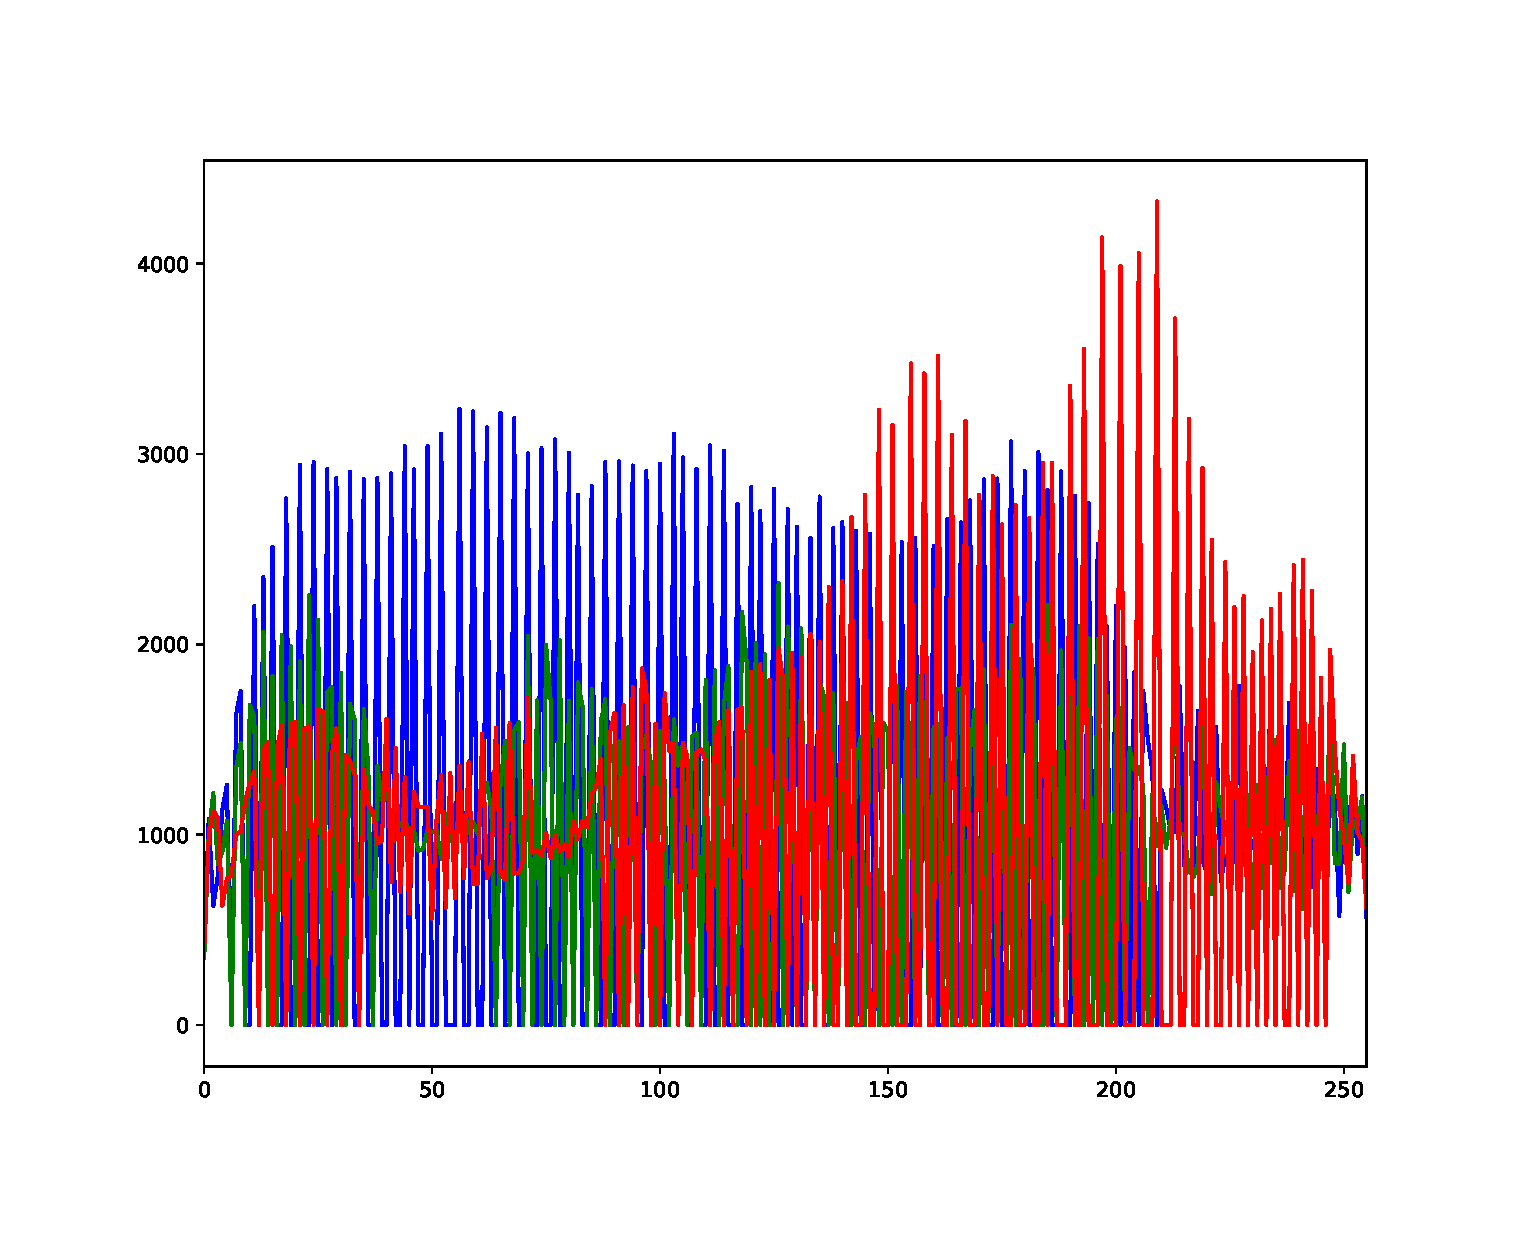
\includegraphics[scale=0.2]{figures/hisequ}
		
	}
	\caption{Histogram computation and Histogram equalization}
\end{figure}    
    
    \begin{tcolorbox}[breakable, size=fbox, boxrule=1pt, pad at break*=1mm,colback=cellbackground, colframe=cellborder]
\prompt{In}{incolor}{1}{\boxspacing}
\begin{Verbatim}[commandchars=\\\{\}]
\PY{n}{channels} \PY{o}{=} \PY{p}{[}\PY{l+s+s1}{\PYZsq{}}\PY{l+s+s1}{b}\PY{l+s+s1}{\PYZsq{}}\PY{p}{,} \PY{l+s+s1}{\PYZsq{}}\PY{l+s+s1}{g}\PY{l+s+s1}{\PYZsq{}}\PY{p}{,} \PY{l+s+s1}{\PYZsq{}}\PY{l+s+s1}{r}\PY{l+s+s1}{\PYZsq{}}\PY{p}{]}\PY{c+c1}{\PYZsh{} since opencv reads img as BGR channel order}
\PY{k}{for} \PY{n}{i}\PY{p}{,} \PY{n}{channel} \PY{o+ow}{in} \PY{n+nb}{enumerate}\PY{p}{(}\PY{n}{channels}\PY{p}{)}\PY{p}{:}
    \PY{n}{histogram} \PY{o}{=} \PY{n}{cv}\PY{o}{.}\PY{n}{calcHist}\PY{p}{(}\PY{p}{[}\PY{n}{img}\PY{p}{]}\PY{p}{,} \PY{p}{[}\PY{n}{i}\PY{p}{]}\PY{p}{,} \PY{k+kc}{None}\PY{p}{,} \PY{p}{[}\PY{l+m+mi}{256}\PY{p}{]}\PY{p}{,} \PY{p}{[}\PY{l+m+mi}{0}\PY{p}{,}\PY{l+m+mi}{256}\PY{p}{]}\PY{p}{)}\PY{c+c1}{\PYZsh{} Calculating Histogram of each channel.}
\PY{n}{equalized\PYZus{}channels} \PY{o}{=} \PY{p}{[}\PY{p}{]}
\PY{k}{for} \PY{n}{channel} \PY{o+ow}{in} \PY{n}{cv}\PY{o}{.}\PY{n}{split}\PY{p}{(}\PY{n}{img}\PY{p}{)}\PY{p}{:}   
    \PY{n}{equalized\PYZus{}channels}\PY{o}{.}\PY{n}{append}\PY{p}{(}\PY{n}{cv}\PY{o}{.}\PY{n}{equalizeHist}\PY{p}{(}\PY{n}{channel}\PY{p}{)}\PY{p}{)}\PY{c+c1}{\PYZsh{} Each channel must be equalized seperately.} 
\PY{n}{equalized\PYZus{}img} \PY{o}{=} \PY{n}{cv}\PY{o}{.}\PY{n}{merge}\PY{p}{(}\PY{n}{equalized\PYZus{}channels}\PY{p}{)}    
\end{Verbatim}
\end{tcolorbox}

\subsection{Intensity transformations}
Intensity transformations is basically a look up table operation. It maps each pixel's intensity to some other intensity depending on a predefined transformation function which only depends on the pixel of interest. Following figures illustrates a transformation consists of three sections(\textit{piece-wise continuous function}). It maps intensities in the ranges [0, 99],[100, 129] and [130, 255] into the ranges [0, 40], [41, 200] and [201, 255] respectively as shown in the transformation function. This kind of transformation is called as \textbf{\textit{Intensity windowing.}}

\begin{figure}[!h]
	\centering
	\subfigure[Original Image]
	{ \includegraphics[scale=0.2]{figures/boriginal}
		
	}
	\subfigure[Transformation]
	{ 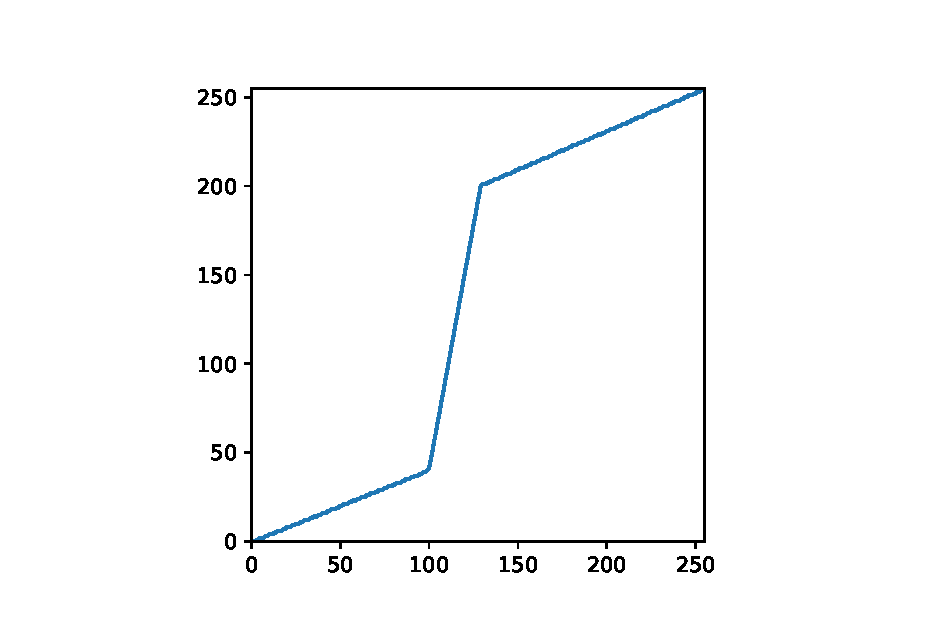
\includegraphics[scale=0.4]{figures/transformation}
		
	}
	\subfigure[Transformed Image]
	{ \includegraphics[scale=0.2]{figures/btransformed}
		
	}
	\caption{Intensity transformations}
\end{figure}

    \begin{tcolorbox}[breakable, size=fbox, boxrule=1pt, pad at break*=1mm,colback=cellbackground, colframe=cellborder]
\prompt{In}{incolor}{2}{\boxspacing}
\begin{Verbatim}[commandchars=\\\{\}]
\PY{n}{a}\PY{p}{,} \PY{n}{b} \PY{o}{=} \PY{p}{[}\PY{l+m+mi}{40}\PY{p}{,}\PY{l+m+mi}{200}\PY{p}{]}
\PY{n}{tr1} \PY{o}{=} \PY{n}{np}\PY{o}{.}\PY{n}{linspace}\PY{p}{(}\PY{l+m+mi}{0}\PY{p}{,}\PY{n}{a}\PY{p}{,}\PY{l+m+mi}{100}\PY{p}{)}\PY{o}{.}\PY{n}{astype}\PY{p}{(}\PY{l+s+s1}{\PYZsq{}}\PY{l+s+s1}{uint8}\PY{l+s+s1}{\PYZsq{}}\PY{p}{)}\PY{c+c1}{\PYZsh{} Declaring tranformations for each region}
\PY{n}{tr2} \PY{o}{=} \PY{n}{np}\PY{o}{.}\PY{n}{linspace}\PY{p}{(}\PY{n}{a}\PY{o}{+}\PY{l+m+mi}{1}\PY{p}{,}\PY{n}{b}\PY{p}{,}\PY{l+m+mi}{30}\PY{p}{)}\PY{o}{.}\PY{n}{astype}\PY{p}{(}\PY{l+s+s1}{\PYZsq{}}\PY{l+s+s1}{uint8}\PY{l+s+s1}{\PYZsq{}}\PY{p}{)}
\PY{n}{tr3} \PY{o}{=} \PY{n}{np}\PY{o}{.}\PY{n}{linspace}\PY{p}{(}\PY{n}{b}\PY{o}{+}\PY{l+m+mi}{1}\PY{p}{,}\PY{l+m+mi}{255}\PY{p}{,}\PY{l+m+mi}{126}\PY{p}{)}\PY{o}{.}\PY{n}{astype}\PY{p}{(}\PY{l+s+s1}{\PYZsq{}}\PY{l+s+s1}{uint8}\PY{l+s+s1}{\PYZsq{}}\PY{p}{)}
\PY{n}{transf} \PY{o}{=} \PY{n}{np}\PY{o}{.}\PY{n}{concatenate}\PY{p}{(}\PY{p}{(}\PY{n}{tr1}\PY{p}{,} \PY{n}{tr2}\PY{p}{)}\PY{p}{,} \PY{n}{axis} \PY{o}{=} \PY{l+m+mi}{0}\PY{p}{)}\PY{c+c1}{\PYZsh{} Concatenating above transfer functions}
\PY{n}{transf} \PY{o}{=} \PY{n}{np}\PY{o}{.}\PY{n}{concatenate}\PY{p}{(}\PY{p}{(}\PY{n}{transf}\PY{p}{,} \PY{n}{tr3}\PY{p}{)}\PY{p}{,} \PY{n}{axis} \PY{o}{=} \PY{l+m+mi}{0}\PY{p}{)}
\PY{n}{transformed\PYZus{}img} \PY{o}{=} \PY{n}{cv}\PY{o}{.}\PY{n}{LUT}\PY{p}{(}\PY{n}{img}\PY{p}{,} \PY{n}{transf}\PY{p}{)}\PY{c+c1}{\PYZsh{} Apply Transformation}
\end{Verbatim}
\end{tcolorbox}

\subsection{Gamma correction}
Image transformation Depends on the value of $\gamma$ as follows,
\begin{itemize}
	\item If $0< \gamma <1$, then function maps narrow range of dark pixels to a wider range of dark pixels which increases the brightness of the image as depicted in figures (c) and (d).

	\item If $\gamma >1$, then opposite of the above process happens and it makes the image darker as in the figure (a).
\end{itemize}
\begin{figure}[!h]
	\centering
	\subfigure[Gamma Corrected Image $\gamma = 1.3$]
	{ \includegraphics[scale=0.2]{figures/dgamma3}
		
	}
	\subfigure[Original Image  $\gamma = 1$]
	{ \includegraphics[scale=0.2]{figures/doriginal}
		
	}
	\subfigure[Gamma Corrected Image $\gamma = 0.7$]
	{ \includegraphics[scale=0.2]{figures/dgamma7}
		
	}
	\subfigure[Gamma Corrected Image $\gamma = 0.4$]
	{ \includegraphics[scale=0.2]{figures/dgamma4}
		
	}
	\caption{Gamma correction}
\end{figure}

    \begin{tcolorbox}[breakable, size=fbox, boxrule=1pt, pad at break*=1mm,colback=cellbackground, colframe=cellborder]
\prompt{In}{incolor}{3}{\boxspacing}
\begin{Verbatim}[commandchars=\\\{\}]
\PY{k}{def} \PY{n+nf}{gammacorrect}\PY{p}{(}\PY{n}{image}\PY{p}{,} \PY{n}{gamma}\PY{p}{)}\PY{p}{:}
    \PY{c+c1}{\PYZsh{} Calculating the lookup table for a given gamma value.}
    \PY{n}{table} \PY{o}{=} \PY{n}{np}\PY{o}{.}\PY{n}{array}\PY{p}{(}\PY{p}{[}\PY{p}{(}\PY{n}{i}\PY{o}{/}\PY{l+m+mf}{255.0}\PY{p}{)}\PY{o}{*}\PY{o}{*}\PY{p}{(}\PY{n}{gamma}\PY{p}{)}\PY{o}{*}\PY{l+m+mf}{255.0} \PY{k}{for} \PY{n}{i} \PY{o+ow}{in} \PY{n}{np}\PY{o}{.}\PY{n}{arange}\PY{p}{(}\PY{l+m+mi}{0}\PY{p}{,}\PY{l+m+mi}{256}\PY{p}{)}\PY{p}{]}\PY{p}{)}\PY{o}{.}\PY{n}{astype}\PY{p}{(}\PY{l+s+s1}{\PYZsq{}}\PY{l+s+s1}{uint8}\PY{l+s+s1}{\PYZsq{}}\PY{p}{)}
    \PY{n}{img\PYZus{}gamma} \PY{o}{=} \PY{n}{cv}\PY{o}{.}\PY{n}{LUT}\PY{p}{(}\PY{n}{image}\PY{p}{,} \PY{n}{table}\PY{p}{)}
    \PY{k}{return} \PY{n}{img\PYZus{}gamma}
\end{Verbatim}
\end{tcolorbox}


\subsection{Gaussian smoothing $\sigma = 1.5$}
Gaussian smoothing is used to reduce sharp transitions in intensities in images(blurring). The extent of blurring depends on both the kernel size and the standard deviation $\sigma$. Each pixel's value is recalculated as the weighted sum of its neighbor pixels where weights are determined by the Gaussian Normal function. Weight decreases as the distance between central pixel and a given pixel increases. Also if the $\sigma$ increases, weights given to the neighbor pixels increases and their contribution to determine the central pixel value increases which makes the image more blur. The effect of kernel size is depicted in the following figures. As kernel size increase more pixels contribute to the calculation of central pixel's value which makes the image more blur.

\begin{figure}[!h]
	\centering
	\subfigure[Original Image]
	{ \includegraphics[scale=0.45]{figures/eoriginal}
		
	}
	\subfigure[Kernel Size = 7]
	{ \includegraphics[scale=0.45]{figures/SmoothkernelS7}
		
	}
	\subfigure[Kernel Size = 13]
	{ \includegraphics[scale=0.45]{figures/SmoothkernelS13}
		
	}
	\subfigure[Kernel Size = 21]
	{ \includegraphics[scale=0.45]{figures/SmoothkernelS21}
		
	}
	\caption{Gaussian smoothing $\sigma = 1.5$}
\end{figure}

    \begin{tcolorbox}[breakable, size=fbox, boxrule=1pt, pad at break*=1mm,colback=cellbackground, colframe=cellborder]
\prompt{In}{incolor}{4}{\boxspacing}
\begin{Verbatim}[commandchars=\\\{\}]
\PY{k}{def} \PY{n+nf}{gaussianSmooth}\PY{p}{(}\PY{n}{image}\PY{p}{,} \PY{n}{kernelSize}\PY{p}{,} \PY{n}{sigma}\PY{p}{)}\PY{p}{:}
    \PY{n}{max\PYZus{}abs} \PY{o}{=} \PY{n}{np}\PY{o}{.}\PY{n}{floor}\PY{p}{(}\PY{n}{kernelSize}\PY{o}{/}\PY{l+m+mi}{2}\PY{p}{)} \PY{c+c1}{\PYZsh{} If kernelSize = 11}
    \PY{n}{x\PYZus{}range} \PY{o}{=} \PY{n}{np}\PY{o}{.}\PY{n}{arange}\PY{p}{(}\PY{o}{\PYZhy{}}\PY{n}{max\PYZus{}abs}\PY{p}{,}\PY{n}{max\PYZus{}abs} \PY{o}{+}\PY{l+m+mi}{1}\PY{p}{,}\PY{l+m+mi}{1}\PY{p}{)} \PY{c+c1}{\PYZsh{}(from \PYZhy{}5 to +5 range)}
    \PY{n}{y\PYZus{}range} \PY{o}{=} \PY{n}{np}\PY{o}{.}\PY{n}{arange}\PY{p}{(}\PY{o}{\PYZhy{}}\PY{n}{max\PYZus{}abs}\PY{p}{,}\PY{n}{max\PYZus{}abs} \PY{o}{+}\PY{l+m+mi}{1}\PY{p}{,}\PY{l+m+mi}{1}\PY{p}{)} \PY{c+c1}{\PYZsh{}(from \PYZhy{}5 to +5 range)}
    \PY{n}{X}\PY{p}{,}\PY{n}{Y} \PY{o}{=} \PY{n}{np}\PY{o}{.}\PY{n}{meshgrid}\PY{p}{(}\PY{n}{x\PYZus{}range}\PY{p}{,} \PY{n}{y\PYZus{}range}\PY{p}{)}
    \PY{n}{kernel} \PY{o}{=} \PY{n}{np}\PY{o}{.}\PY{n}{exp}\PY{p}{(}\PY{p}{(}\PY{o}{\PYZhy{}}\PY{p}{(}\PY{n}{X}\PY{o}{*}\PY{o}{*}\PY{l+m+mi}{2} \PY{o}{+} \PY{n}{Y}\PY{o}{*}\PY{o}{*}\PY{l+m+mi}{2}\PY{p}{)}\PY{p}{)}\PY{o}{/}\PY{p}{(}\PY{l+m+mi}{2}\PY{o}{*}\PY{n}{sigma}\PY{o}{*}\PY{o}{*}\PY{l+m+mi}{2}\PY{p}{)}\PY{p}{)}\PY{o}{/}\PY{p}{(}\PY{l+m+mi}{2}\PY{o}{*}\PY{n}{np}\PY{o}{.}\PY{n}{pi}\PY{o}{*}\PY{n}{sigma}\PY{o}{*}\PY{o}{*}\PY{l+m+mi}{2}\PY{p}{)}\PY{c+c1}{\PYZsh{} Bulding Gaussian kernel}
    \PY{n}{smoothed\PYZus{}img} \PY{o}{=} \PY{n}{cv}\PY{o}{.}\PY{n}{filter2D}\PY{p}{(}\PY{n}{image}\PY{p}{,}\PY{o}{\PYZhy{}}\PY{l+m+mi}{1}\PY{p}{,}\PY{n}{kernel}\PY{p}{)}\PY{c+c1}{\PYZsh{} Convolution of the image with the kernel}
    \PY{k}{return} \PY{n}{smoothed\PYZus{}img}
\end{Verbatim}
\end{tcolorbox}

\subsection{Unsharp masking}
Unsharp masking is an image sharpening method which is used to highlight intensity transitions in the image. It has following three main steps as depicted in the figures. \textbf{(1.)} Original image is blurred using an averaging kernel(\textit{here Gaussian kernel is used.}). \textbf{(2.)} Blurred image is subtracted form the original image to obtain the ``mask''. \textbf{(3.)} ``Mask'' is then added to the original image to obtain the sharpened image. To eliminate overflow occurs in the addition of two images OpenCV's {\tt addWeighted} function is used.

\begin{figure}[!h]
	\centering
	\subfigure[Original Image]
	{ \includegraphics[scale=0.25]{figures/foriginal}
		
	}
	\subfigure[Gaussian Blurred]
	{ \includegraphics[scale=0.25]{figures/blurred}
		
	}
	\subfigure[Mask + 125]
	{ \includegraphics[scale=0.25]{figures/mask}
		
	}
	\subfigure[Sharpened Image]
	{ \includegraphics[scale=0.25]{figures/sharpened}
		
	}
	\caption{Unsharp masking}
\end{figure}

    \begin{tcolorbox}[breakable, size=fbox, boxrule=1pt, pad at break*=1mm,colback=cellbackground, colframe=cellborder]
\prompt{In}{incolor}{5}{\boxspacing}
\begin{Verbatim}[commandchars=\\\{\}]
\PY{n}{sigma} \PY{o}{=} \PY{l+m+mi}{2} 
\PY{n}{kernel} \PY{o}{=} \PY{n}{cv}\PY{o}{.}\PY{n}{getGaussianKernel}\PY{p}{(}\PY{l+m+mi}{5}\PY{p}{,} \PY{n}{sigma}\PY{p}{)} \PY{c+c1}{\PYZsh{}create the gaussian kernel}
\PY{n}{blurred} \PY{o}{=} \PY{n}{cv}\PY{o}{.}\PY{n}{sepFilter2D}\PY{p}{(}\PY{n}{img}\PY{p}{,} \PY{o}{\PYZhy{}}\PY{l+m+mi}{1}\PY{p}{,} \PY{n}{kernel}\PY{p}{,} \PY{n}{kernel}\PY{p}{,} \PY{n}{anchor}\PY{o}{=}\PY{p}{(}\PY{o}{\PYZhy{}}\PY{l+m+mi}{1}\PY{p}{,}\PY{o}{\PYZhy{}}\PY{l+m+mi}{1}\PY{p}{)}\PY{p}{,} \PY{n}{delta}\PY{o}{=}\PY{l+m+mi}{0}\PY{p}{,} \PY{n}{borderType}\PY{o}{=}\PY{n}{cv}\PY{o}{.}\PY{n}{BORDER\PYZus{}REPLICATE}\PY{p}{)}
\PY{n}{mask} \PY{o}{=} \PY{n}{img}\PY{o}{.}\PY{n}{astype}\PY{p}{(}\PY{l+s+s1}{\PYZsq{}}\PY{l+s+s1}{float32}\PY{l+s+s1}{\PYZsq{}}\PY{p}{)} \PY{o}{\PYZhy{}} \PY{n}{blurred}\PY{o}{.}\PY{n}{astype}\PY{p}{(}\PY{l+s+s1}{\PYZsq{}}\PY{l+s+s1}{float32}\PY{l+s+s1}{\PYZsq{}}\PY{p}{)}
\PY{n}{k} \PY{o}{=} \PY{l+m+mi}{1} \PY{c+c1}{\PYZsh{} when k =1 : unsharp masking, when k\PYZgt{}1 : Highboost Filtering}
\PY{n}{sharpened} \PY{o}{=} \PY{n}{cv}\PY{o}{.}\PY{n}{addWeighted}\PY{p}{(}\PY{n}{img}\PY{o}{.}\PY{n}{astype}\PY{p}{(}\PY{l+s+s1}{\PYZsq{}}\PY{l+s+s1}{float32}\PY{l+s+s1}{\PYZsq{}}\PY{p}{)} \PY{p}{,} \PY{l+m+mf}{1.}\PY{p}{,} \PY{n}{mask}\PY{p}{,} \PY{n}{k}\PY{p}{,} \PY{l+m+mi}{0}\PY{p}{)}
\end{Verbatim}
\end{tcolorbox}

\subsection{Median filtering }
Non-linear Median filter is heavily used to remove random noises like salt and pepper noise from images due to its excellence  noise-reduction capability over any other averaging filter. As its name implies it replaces value of the central pixel by the median of the intensity values in the neighborhood of that pixel. As following figures depict noise in the figure (b) is completely removed by a $5 \times 5$ median filter which is not possible with an averaging filter like Gaussian.

\begin{figure}[!h]
	\centering
	\subfigure[Original Image]
	{ \includegraphics[scale=0.23]{figures/goriginal}
		
	}
	\subfigure[Adding Salt \& Pepper Noise]
	{ \includegraphics[scale=0.23]{figures/saltpepper}
		
	}
	\subfigure[Kernel Size = 3]
	{ \includegraphics[scale=0.23]{figures/medianfilterimage3}
		
	}
	\subfigure[Kernel Size = 5]
	{ \includegraphics[scale=0.23]{figures/medianfilterimage5}
		
	}
	\caption{Median filtering }
\end{figure}

    \begin{tcolorbox}[breakable, size=fbox, boxrule=1pt, pad at break*=1mm,colback=cellbackground, colframe=cellborder]
\prompt{In}{incolor}{6}{\boxspacing}
\begin{Verbatim}[commandchars=\\\{\}]
\PY{n}{saltpepper} \PY{o}{=} \PY{n}{noisy}\PY{p}{(}\PY{l+s+s2}{\PYZdq{}}\PY{l+s+s2}{s\PYZam{}p}\PY{l+s+s2}{\PYZdq{}}\PY{p}{,} \PY{n}{img}\PY{p}{)}\PY{c+c1}{\PYZsh{} noise generated using noisy fun @:stackoverflow.com/a/30609854}
\PY{n}{kernelSize} \PY{o}{=} \PY{l+m+mi}{3}
\PY{n}{medianfiltered\PYZus{}image} \PY{o}{=} \PY{n}{cv}\PY{o}{.}\PY{n}{medianBlur}\PY{p}{(}\PY{n}{saltpepper}\PY{p}{,} \PY{n}{kernelSize}\PY{p}{)} 
\end{Verbatim}
\end{tcolorbox}

\subsection{Bilateral filtering}

Bilateral filter extends the idea of Gaussian smoothing by adding \textbf{\textit{edge preserving capability}} which is not possible in the Gaussian filtering because there, only the Spatial distance to the pixels' from the central pixel were considered when applying the weights(\textit{Same Gaussian kernel everywhere regardless of the pixel's intensity}) and therefore \textbf{\textit{Gaussian filter averages across the edges}} assuming that pixels' intensity value do not change rapidly over the window. As a consequence the same weight may be applied to a pixel on an edge(say high intensity) and a pixel near an edge(say low intensity) when calculating the central pixel's value of a window centered at a pixel near an edge.\\

In the bilateral filter \textbf{\textit{intensities of the neighborhood pixels are also considered}} when applying the weights, in addition to the spatial distance. This makes it possible to \textbf{\textit{eliminate the averaging across edges}}. As following figures shows when $\sigma_r$ approaches $\infty$, bilateral filter gives the result of the Gaussian filter. Here $\sigma_s$ is spatial deviation(\textit{spatial extent of the kernel}) while $\sigma_r$ is the color space deviation(\textit{minimum amplitude of an edge}).
\begin{figure}[!h]
	\centering
	\subfigure[Original Image]
	{ \includegraphics[scale=0.37]{figures/horiginal}
		
	}
	\subfigure[Gaussian Kernel Size = 9, $\sigma_s=6$]
	{ \includegraphics[scale=0.37]{figures/gaussianB}
		
	}
	\subfigure[Bilateral Kernel Size = 9, $\sigma_s = 6$, $\sigma_r = 100$ ]
	{ \includegraphics[scale=0.37]{figures/bl5}
	}
	\subfigure[Bilateral Kernel Size = 13, $\sigma_s = 6$, $\sigma_r = 10$]
	{ \includegraphics[scale=0.37]{figures/bl9}
	}
	\caption{Bilateral filtering}
\end{figure}

    \begin{tcolorbox}[breakable, size=fbox, boxrule=1pt, pad at break*=1mm,colback=cellbackground, colframe=cellborder]
\prompt{In}{incolor}{7}{\boxspacing}
\begin{Verbatim}[commandchars=\\\{\}]
\PY{c+c1}{\PYZsh{}dst = cv.bilateralFilter(src, d(KernelSize), sigmaColor, sigmaSpace)}
\PY{n}{bilateral1} \PY{o}{=} \PY{n}{cv}\PY{o}{.}\PY{n}{bilateralFilter}\PY{p}{(}\PY{n}{img}\PY{p}{,}\PY{l+m+mi}{9}\PY{p}{,}\PY{l+m+mi}{100}\PY{p}{,}\PY{l+m+mi}{6}\PY{p}{)}\PY{c+c1}{\PYZsh{} Edges are blurred. Almost Gaussian} 
\PY{n}{bilateral2} \PY{o}{=} \PY{n}{cv}\PY{o}{.}\PY{n}{bilateralFilter}\PY{p}{(}\PY{n}{img}\PY{p}{,}\PY{l+m+mi}{13}\PY{p}{,}\PY{l+m+mi}{10}\PY{p}{,}\PY{l+m+mi}{6}\PY{p}{)}\PY{c+c1}{\PYZsh{} Edges are preserved} 
\end{Verbatim}
\end{tcolorbox}

\vspace{5mm}
\hrule

\section{Part 2: Count the rice grains in the rice image}

The objective of counting the rice grains can be achieved through binary segmentation as we have only two different object types namely rice grains and the background. Since the image has different lighting conditions, \textbf{\textit{adaptive thresholding}} must be used for binary segmentation. Optimum parameter values for the thresholding function was obtained though trial and error. To get rid of the unwanted white noise in the background and to detach connected grains as depicted in the figure (b) \textbf{\textit{erosion morphological transformation}} is used(\textit{Rectangular kernel is used over elliptic and cross shape kernels since it was found to be the best at achieving the aforementioned requirements}).\\

After the above post-processing what is left is just to count the distinct white objects(rice grains) in the figure (c). For that Connected Components Analysis(CCA) is used. It gives each distinct grain a distinct label(\textit{an integer starting form 0(for background) to some number}). This can be done through OpenCV's {\tt connectedComponents} function which returns total number of labels and the labeled image. Since this total number of labels includes the background as well, we need to subtract 1 from it to get the grain  count. All the components in the labeled image can be easily visualized through a proper color map as depicted in figure (e). Before map the colors, figure (d) is normalized to get a uniform intensity distribution in the range[0, 255] which makes the color mapping more distributed.\\

{\tt Through the following algorithm it was found that there are 100 grains in the given image.}

\begin{figure}[!h]
	\centering
	\subfigure[Gray Scale Image]
	{ \includegraphics[scale=0.38]{figures/part2/2original}
	}
	\subfigure[Adaptive Thresholding]
	{ \includegraphics[scale=0.38]{figures/part2/img_adapt_thresh}
	}
	\subfigure[Erosion]
	{ \includegraphics[scale=0.38]{figures/part2/eroded_img}
	}
	\subfigure[Connected Components]
	{ \includegraphics[scale=0.38]{figures/part2/labeledImg}
	}
	\subfigure[Color Mapped Image]
	{ \includegraphics[scale=0.38]{figures/part2/imgColorMap}
	}
	\caption{Counting the rice grains}
\end{figure}

    \begin{tcolorbox}[breakable, size=fbox, boxrule=1pt, pad at break*=1mm,colback=cellbackground, colframe=cellborder]
\prompt{In}{incolor}{8}{\boxspacing}
\begin{Verbatim}[commandchars=\\\{\}]
\PY{c+c1}{\PYZsh{} reading the image as an eight bit grayscale image}
\PY{n}{img} \PY{o}{=} \PY{n}{cv}\PY{o}{.}\PY{n}{imread}\PY{p}{(}\PY{l+s+s2}{\PYZdq{}}\PY{l+s+s2}{../a01images/rice.png}\PY{l+s+s2}{\PYZdq{}}\PY{p}{,} \PY{n}{cv}\PY{o}{.}\PY{n}{IMREAD\PYZus{}GRAYSCALE}\PY{p}{)}
\PY{c+c1}{\PYZsh{} adaptive thresholding due to non uniform illumination in the image}
\PY{n}{kernelSize}\PY{p}{,} \PY{n}{C} \PY{o}{=} \PY{l+m+mi}{25}\PY{p}{,}\PY{o}{\PYZhy{}}\PY{l+m+mi}{10}
\PY{n}{img\PYZus{}adapt\PYZus{}thresh} \PY{o}{=} \PY{n}{th2} \PY{o}{=} \PY{n}{cv}\PY{o}{.}\PY{n}{adaptiveThreshold}\PY{p}{(}\PY{n}{img}\PY{p}{,}\PY{l+m+mi}{255}\PY{p}{,}\PY{n}{cv}\PY{o}{.}\PY{n}{ADAPTIVE\PYZus{}THRESH\PYZus{}MEAN\PYZus{}C}\PY{p}{,} \PY{n}{cv}\PY{o}{.}\PY{n}{THRESH\PYZus{}BINARY}\PY{p}{,}\PY{n}{kernelSize}\PY{p}{,} \PY{n}{C}\PY{p}{)}
\PY{c+c1}{\PYZsh{} Morphological transf: Erosion to eliminate white noise and detach connected objects}
\PY{n}{ksize} \PY{o}{=} \PY{l+m+mi}{3}
\PY{n}{kernel} \PY{o}{=} \PY{n}{cv}\PY{o}{.}\PY{n}{getStructuringElement}\PY{p}{(}\PY{n}{cv}\PY{o}{.}\PY{n}{MORPH\PYZus{}RECT}\PY{p}{,}\PY{p}{(}\PY{n}{ksize}\PY{p}{,}\PY{n}{ksize}\PY{p}{)}\PY{p}{)}
\PY{n}{eroded\PYZus{}img} \PY{o}{=} \PY{n}{cv}\PY{o}{.}\PY{n}{erode}\PY{p}{(}\PY{n}{img\PYZus{}adapt\PYZus{}thresh}\PY{p}{,} \PY{n}{kernel}\PY{p}{)}
\PY{c+c1}{\PYZsh{}\PYZhy{}\PYZhy{}\PYZhy{}\PYZhy{}\PYZhy{}\PYZhy{}\PYZhy{}\PYZhy{}\PYZhy{}\PYZhy{}\PYZhy{}\PYZhy{}\PYZhy{}\PYZhy{}\PYZhy{}\PYZhy{}\PYZhy{}Connected components Analysis(CCA)\PYZhy{}\PYZhy{}\PYZhy{}\PYZhy{}\PYZhy{}\PYZhy{}\PYZhy{}\PYZhy{}\PYZhy{}\PYZhy{}\PYZhy{}\PYZhy{}\PYZhy{}\PYZhy{}\PYZhy{}\PYZhy{}\PYZhy{}\PYZhy{}\PYZhy{}\PYZhy{}\PYZhy{}\PYZhy{}}
\PY{n}{num\PYZus{}labels}\PY{p}{,} \PY{n}{labeledImg} \PY{o}{=} \PY{n}{cv}\PY{o}{.}\PY{n}{connectedComponents}\PY{p}{(}\PY{n}{eroded\PYZus{}img}\PY{p}{)}
\PY{c+c1}{\PYZsh{} Background is considered as another object in CCA. Therfore it needs to be subtracted}
\PY{n}{num\PYZus{}grains} \PY{o}{=} \PY{n}{num\PYZus{}labels} \PY{o}{\PYZhy{}}\PY{l+m+mi}{1}\PY{p}{;} \PY{n+nb}{print}\PY{p}{(}\PY{n}{num\PYZus{}grains}\PY{p}{)}
\PY{c+c1}{\PYZsh{}\PYZhy{}\PYZhy{}\PYZhy{}\PYZhy{}\PYZhy{}\PYZhy{}\PYZhy{}\PYZhy{}\PYZhy{}\PYZhy{}\PYZhy{}\PYZhy{}\PYZhy{}\PYZhy{}\PYZhy{}\PYZhy{}\PYZhy{}Show components using a color Map.\PYZhy{}\PYZhy{}\PYZhy{}\PYZhy{}\PYZhy{}\PYZhy{}\PYZhy{}\PYZhy{}\PYZhy{}\PYZhy{}\PYZhy{}\PYZhy{}\PYZhy{}\PYZhy{}\PYZhy{}\PYZhy{}\PYZhy{}\PYZhy{}\PYZhy{}\PYZhy{}\PYZhy{}\PYZhy{}}
\PY{p}{(}\PY{n}{minVal}\PY{p}{,} \PY{n}{maxVal}\PY{p}{,} \PY{n}{minLoc}\PY{p}{,} \PY{n}{maxLoc}\PY{p}{)} \PY{o}{=} \PY{n}{cv}\PY{o}{.}\PY{n}{minMaxLoc}\PY{p}{(}\PY{n}{labeledImg}\PY{p}{)}\PY{c+c1}{\PYZsh{} find min,max pixel values \& locations }
\PY{n}{labeledImg} \PY{o}{=} \PY{p}{(}\PY{l+m+mi}{255}\PY{o}{/}\PY{p}{(}\PY{n}{maxVal}\PY{o}{\PYZhy{}}\PY{n}{minVal}\PY{p}{)}\PY{p}{)} \PY{o}{*} \PY{p}{(}\PY{n}{labeledImg} \PY{o}{\PYZhy{}} \PY{n}{minVal}\PY{p}{)}\PY{c+c1}{\PYZsh{} Normalizing image so, min= 0 \& max = 255.}
\PY{n}{imgColorMap} \PY{o}{=} \PY{n}{cv}\PY{o}{.}\PY{n}{applyColorMap}\PY{p}{(}\PY{n}{labeledImg}\PY{o}{.}\PY{n}{astype}\PY{p}{(}\PY{l+s+s1}{\PYZsq{}}\PY{l+s+s1}{uint8}\PY{l+s+s1}{\PYZsq{}}\PY{p}{)}\PY{p}{,} \PY{n}{cv}\PY{o}{.}\PY{n}{COLORMAP\PYZus{}RAINBOW}\PY{p}{)}\PY{c+c1}{\PYZsh{} Applying color map}
\PY{n}{imgColorMap}\PY{p}{[}\PY{n}{labeledImg}\PY{o}{==}\PY{l+m+mi}{0}\PY{p}{]} \PY{o}{=} \PY{l+m+mi}{0}\PY{c+c1}{\PYZsh{} Making the background black}
\PY{n}{plt}\PY{o}{.}\PY{n}{imshow}\PY{p}{(}\PY{n}{imgColorMap}\PY{p}{[}\PY{p}{:}\PY{p}{,}\PY{p}{:}\PY{p}{,}\PY{p}{:}\PY{p}{:}\PY{o}{\PYZhy{}}\PY{l+m+mi}{1}\PY{p}{]}\PY{p}{)}\PY{c+c1}{\PYZsh{} Display colormapped labels}
\end{Verbatim}
\end{tcolorbox}

\vspace{5mm}
\hrule
\section{Part 3: Zoom Images}        

Following code implements \textbf{\textit{Nearest Neighbor}} and \textbf{\textit{Bi-linear Interpolation}}  methods of image zooming. As following figure depicts bi-linear interpolation method is better than nearest neighbor method since it interpolates each pixel's intensity value using its neighbors' values rather than simply taking the nearest neighbor's value when assigning values to the pixels in the zoomed image. Because of this reason continuous nature of intensities is violated  and pixel's rectangular structure is clearly visible in the image, zoomed using the nearest neighbor method which is not the case in the bi-linear interpolation method.

\begin{figure}[!h]
	\centering
	\subfigure[Nearest Neighbor Method]
	{ \includegraphics[scale=0.85]{figures/part3/zoomedImgnncrop}
	}
	\subfigure[Bilinear Interpolation Method]
	{ \includegraphics[scale=0.825]{figures/part3/zoomedImgbicrop}
	}
	\caption{Zooming Images}
\end{figure}

These two methods can be easily explained using a count example as follows. Consider a pixel in a zoomed image($1920 \times1200$) whose coordinates are ($235,526$). Assume this image was obtained by scaling an image($480\times300$) by a factor of 4.

\begin{itemize}
	\item First step is common to the both methods, that is calculating the corresponding pixel in the original source image by dividing the coordinates by the scaling factor. Therefore source coordinates = ($235/4,526/4$) = ($58.75, 131.5$)
	\item In the {\tt Nearest Neighbor Method} these coordinates are rounded to the nearest integers within the source image dimensions. Then corresponding pixel in the source image = ($59, 132$) and intensity of that pixel is assigned to the pixel($235,526$) in the zoomed image.
	\item But in the {\tt Bi-linear Interpolation Method} it considers intensities of all of its neighbors. That is intensities of, ($58, 131$),($58, 132$),($59, 131$) and ($59, 132$) are considered and it interpolates the intensity of an imaginary pixel at the coordinates($58.75, 131.5$) using those intensities. That intensity value is then assigned to the corresponding pixel($235,526$) in the zoomed image.
\end{itemize}

Because of this difference in  intensity assigning procedure, Bi-linear Interpolation Method is computationally expensive and its quality is much better than the Nearest Neighbor Method. 
\vfill  
    \begin{tcolorbox}[breakable, size=fbox, boxrule=1pt, pad at break*=1mm,colback=cellbackground, colframe=cellborder]
\prompt{In}{incolor}{9}{\boxspacing}
\begin{Verbatim}[commandchars=\\\{\}]
\PY{k}{def} \PY{n+nf}{zoom}\PY{p}{(}\PY{n}{image}\PY{p}{,} \PY{n}{scaling\PYZus{}factor}\PY{p}{,} \PY{n}{method}\PY{p}{)}\PY{p}{:}
    \PY{n}{img} \PY{o}{=} \PY{n}{image}
    \PY{n}{sf} \PY{o}{=} \PY{n}{scaling\PYZus{}factor}
    \PY{c+c1}{\PYZsh{} Determining dimensions of the zoomed image}
    \PY{k}{if} \PY{n+nb}{len}\PY{p}{(}\PY{n}{img}\PY{o}{.}\PY{n}{shape}\PY{p}{)} \PY{o}{==} \PY{l+m+mi}{2}\PY{p}{:} \PY{c+c1}{\PYZsh{} for GRAYSCALE images}
        \PY{n}{zoomedImgDims} \PY{o}{=} \PY{p}{[}\PY{n+nb}{int}\PY{p}{(}\PY{n}{dim}\PY{o}{*}\PY{n}{sf}\PY{p}{)} \PY{k}{for} \PY{n}{dim} \PY{o+ow}{in} \PY{n}{img}\PY{o}{.}\PY{n}{shape}\PY{p}{]}
    \PY{k}{else}\PY{p}{:} \PY{c+c1}{\PYZsh{} for COLOR images}
        \PY{n}{zoomedImgDims} \PY{o}{=} \PY{p}{[}\PY{n+nb}{int}\PY{p}{(}\PY{n}{dim}\PY{o}{*}\PY{n}{sf}\PY{p}{)} \PY{k}{for} \PY{n}{dim} \PY{o+ow}{in} \PY{n}{img}\PY{o}{.}\PY{n}{shape}\PY{p}{]}
        \PY{n}{zoomedImgDims}\PY{p}{[}\PY{l+m+mi}{2}\PY{p}{]} \PY{o}{=} \PY{l+m+mi}{3}
    \PY{n}{zoomedImg} \PY{o}{=} \PY{n}{np}\PY{o}{.}\PY{n}{zeros}\PY{p}{(}\PY{n}{zoomedImgDims}\PY{p}{,} \PY{n}{dtype} \PY{o}{=} \PY{n}{img}\PY{o}{.}\PY{n}{dtype}\PY{p}{)}\PY{c+c1}{\PYZsh{} declaring an empty array to store values}
\PY{c+c1}{\PYZsh{}====================Nearest Neighbour Mehtod(NNM)=========================}
    \PY{k}{if} \PY{n}{method} \PY{o}{==} \PY{l+s+s1}{\PYZsq{}}\PY{l+s+s1}{nn}\PY{l+s+s1}{\PYZsq{}}\PY{p}{:}        
        \PY{k}{for} \PY{n}{row} \PY{o+ow}{in} \PY{n+nb}{range}\PY{p}{(}\PY{n}{zoomedImg}\PY{o}{.}\PY{n}{shape}\PY{p}{[}\PY{l+m+mi}{0}\PY{p}{]}\PY{p}{)}\PY{p}{:}
            \PY{n}{source\PYZus{}row} \PY{o}{=} \PY{n+nb}{round}\PY{p}{(}\PY{n}{row}\PY{o}{/}\PY{n}{sf}\PY{p}{)}\PY{c+c1}{\PYZsh{} Calculating corresponding pixels in original image }
            \PY{k}{if} \PY{n}{source\PYZus{}row} \PY{o}{\PYZgt{}} \PY{n}{img}\PY{o}{.}\PY{n}{shape}\PY{p}{[}\PY{l+m+mi}{0}\PY{p}{]}\PY{o}{\PYZhy{}}\PY{l+m+mi}{1}\PY{p}{:} \PY{n}{source\PYZus{}row} \PY{o}{=} \PY{n}{img}\PY{o}{.}\PY{n}{shape}\PY{p}{[}\PY{l+m+mi}{0}\PY{p}{]}\PY{o}{\PYZhy{}}\PY{l+m+mi}{1}\PY{c+c1}{\PYZsh{} Overflow handling}
            \PY{k}{for} \PY{n}{column} \PY{o+ow}{in} \PY{n+nb}{range}\PY{p}{(}\PY{n}{zoomedImg}\PY{o}{.}\PY{n}{shape}\PY{p}{[}\PY{l+m+mi}{1}\PY{p}{]}\PY{p}{)}\PY{p}{:}
                \PY{n}{source\PYZus{}column} \PY{o}{=} \PY{n+nb}{round}\PY{p}{(}\PY{n}{column}\PY{o}{/}\PY{n}{sf}\PY{p}{)}\PY{c+c1}{\PYZsh{} Calculating corresponding pixels in original image}
                \PY{k}{if} \PY{n}{source\PYZus{}column} \PY{o}{\PYZgt{}} \PY{n}{img}\PY{o}{.}\PY{n}{shape}\PY{p}{[}\PY{l+m+mi}{1}\PY{p}{]}\PY{o}{\PYZhy{}}\PY{l+m+mi}{1}\PY{p}{:} \PY{n}{source\PYZus{}column} \PY{o}{=} \PY{n}{img}\PY{o}{.}\PY{n}{shape}\PY{p}{[}\PY{l+m+mi}{1}\PY{p}{]}\PY{o}{\PYZhy{}}\PY{l+m+mi}{1}\PY{c+c1}{\PYZsh{} Overflow handling}
                \PY{c+c1}{\PYZsh{} Assigning pixel values}
                \PY{k}{if} \PY{n+nb}{len}\PY{p}{(}\PY{n}{img}\PY{o}{.}\PY{n}{shape}\PY{p}{)} \PY{o}{==} \PY{l+m+mi}{2}\PY{p}{:}
                    \PY{n}{zoomedImg}\PY{p}{[}\PY{n}{row}\PY{p}{]}\PY{p}{[}\PY{n}{column}\PY{p}{]} \PY{o}{=} \PY{n}{img}\PY{p}{[}\PY{n}{source\PYZus{}row}\PY{p}{]}\PY{p}{[}\PY{n}{source\PYZus{}column}\PY{p}{]}
                \PY{k}{else}\PY{p}{:}
                    \PY{k}{for} \PY{n}{channel} \PY{o+ow}{in} \PY{n+nb}{range}\PY{p}{(}\PY{l+m+mi}{3}\PY{p}{)}\PY{p}{:}
                        \PY{n}{zoomedImg}\PY{p}{[}\PY{n}{row}\PY{p}{]}\PY{p}{[}\PY{n}{column}\PY{p}{]}\PY{p}{[}\PY{n}{channel}\PY{p}{]} \PY{o}{=} \PYZbs{}
                                            \PY{n}{img}\PY{p}{[}\PY{n}{source\PYZus{}row}\PY{p}{]}\PY{p}{[}\PY{n}{source\PYZus{}column}\PY{p}{]}\PY{p}{[}\PY{n}{channel}\PY{p}{]}
\PY{c+c1}{\PYZsh{}======================Bilinear Interpolation Mehtod(BIM)==================     }
    \PY{k}{if} \PY{n}{method} \PY{o}{==} \PY{l+s+s1}{\PYZsq{}}\PY{l+s+s1}{bi}\PY{l+s+s1}{\PYZsq{}}\PY{p}{:}
        \PY{k}{for} \PY{n}{row} \PY{o+ow}{in} \PY{n+nb}{range}\PY{p}{(}\PY{n}{zoomedImg}\PY{o}{.}\PY{n}{shape}\PY{p}{[}\PY{l+m+mi}{0}\PY{p}{]}\PY{p}{)}\PY{p}{:}
            \PY{n}{row\PYZus{}position} \PY{o}{=} \PY{n}{row}\PY{o}{/}\PY{n}{sf}\PY{c+c1}{\PYZsh{} Calculating corresponding row in original image}
            \PY{n}{row\PYZus{}below} \PY{o}{=} \PY{n+nb}{int}\PY{p}{(}\PY{n}{np}\PY{o}{.}\PY{n}{floor}\PY{p}{(}\PY{n}{row\PYZus{}position}\PY{p}{)}\PY{p}{)}
            \PY{n}{row\PYZus{}up} \PY{o}{=} \PY{n+nb}{int}\PY{p}{(}\PY{n}{np}\PY{o}{.}\PY{n}{ceil}\PY{p}{(}\PY{n}{row\PYZus{}position}\PY{p}{)}\PY{p}{)}
            \PY{k}{if} \PY{n}{row\PYZus{}up} \PY{o}{\PYZgt{}} \PY{n}{img}\PY{o}{.}\PY{n}{shape}\PY{p}{[}\PY{l+m+mi}{0}\PY{p}{]}\PY{o}{\PYZhy{}}\PY{l+m+mi}{1}\PY{p}{:} \PY{n}{row\PYZus{}up} \PY{o}{=} \PY{n}{img}\PY{o}{.}\PY{n}{shape}\PY{p}{[}\PY{l+m+mi}{0}\PY{p}{]}\PY{o}{\PYZhy{}}\PY{l+m+mi}{1}\PY{c+c1}{\PYZsh{} Overflow handling}
            \PY{k}{for} \PY{n}{column} \PY{o+ow}{in} \PY{n+nb}{range}\PY{p}{(}\PY{n}{zoomedImg}\PY{o}{.}\PY{n}{shape}\PY{p}{[}\PY{l+m+mi}{1}\PY{p}{]}\PY{p}{)}\PY{p}{:}
                \PY{n}{column\PYZus{}position} \PY{o}{=} \PY{n}{column}\PY{o}{/}\PY{n}{sf}\PY{c+c1}{\PYZsh{} Calculating corresponding column in original image}
                \PY{n}{column\PYZus{}previous} \PY{o}{=} \PY{n+nb}{int}\PY{p}{(}\PY{n}{np}\PY{o}{.}\PY{n}{floor}\PY{p}{(}\PY{n}{column\PYZus{}position}\PY{p}{)}\PY{p}{)}
                \PY{n}{column\PYZus{}next} \PY{o}{=} \PY{n+nb}{int}\PY{p}{(}\PY{n}{np}\PY{o}{.}\PY{n}{ceil}\PY{p}{(}\PY{n}{column\PYZus{}position}\PY{p}{)}\PY{p}{)}
                \PY{k}{if} \PY{n}{column\PYZus{}next} \PY{o}{\PYZgt{}} \PY{n}{img}\PY{o}{.}\PY{n}{shape}\PY{p}{[}\PY{l+m+mi}{1}\PY{p}{]}\PY{o}{\PYZhy{}}\PY{l+m+mi}{1}\PY{p}{:} \PY{n}{column\PYZus{}next} \PY{o}{=} \PY{n}{img}\PY{o}{.}\PY{n}{shape}\PY{p}{[}\PY{l+m+mi}{1}\PY{p}{]}\PY{o}{\PYZhy{}}\PY{l+m+mi}{1}

                \PY{n}{diff1} \PY{o}{=} \PY{n}{row\PYZus{}position} \PY{o}{\PYZhy{}} \PY{n}{row\PYZus{}below} 
                \PY{n}{diff2} \PY{o}{=} \PY{n}{column\PYZus{}position} \PY{o}{\PYZhy{}} \PY{n}{column\PYZus{}previous}
                \PY{k}{if} \PY{n+nb}{len}\PY{p}{(}\PY{n}{img}\PY{o}{.}\PY{n}{shape}\PY{p}{)} \PY{o}{==} \PY{l+m+mi}{2}\PY{p}{:} \PY{c+c1}{\PYZsh{} for GRAYSCALE images}
                    \PY{n}{interVal1} \PY{o}{=} \PY{n}{img}\PY{p}{[}\PY{n}{row\PYZus{}below}\PY{p}{]}\PY{p}{[}\PY{n}{column\PYZus{}previous}\PY{p}{]}\PY{o}{*}\PY{p}{(}\PY{l+m+mi}{1}\PY{o}{\PYZhy{}}\PY{n}{diff1}\PY{p}{)}\PYZbs{}
                                \PY{o}{+} \PY{n}{img}\PY{p}{[}\PY{n}{row\PYZus{}up}\PY{p}{]}\PY{p}{[}\PY{n}{column\PYZus{}previous}\PY{p}{]}\PY{o}{*}\PY{p}{(}\PY{n}{diff1}\PY{p}{)}
                    \PY{n}{interVal2} \PY{o}{=} \PY{n}{img}\PY{p}{[}\PY{n}{row\PYZus{}below}\PY{p}{]}\PY{p}{[}\PY{n}{column\PYZus{}next}\PY{p}{]}\PY{o}{*}\PY{p}{(}\PY{l+m+mi}{1}\PY{o}{\PYZhy{}}\PY{n}{diff1}\PY{p}{)}\PYZbs{}
                                \PY{o}{+} \PY{n}{img}\PY{p}{[}\PY{n}{row\PYZus{}up}\PY{p}{]}\PY{p}{[}\PY{n}{column\PYZus{}next}\PY{p}{]}\PY{o}{*}\PY{p}{(}\PY{n}{diff1}\PY{p}{)}
                    \PY{n}{zoomedImg}\PY{p}{[}\PY{n}{row}\PY{p}{]}\PY{p}{[}\PY{n}{column}\PY{p}{]} \PY{o}{=} \PY{p}{(}\PY{n}{interVal1}\PY{o}{*}\PY{p}{(}\PY{l+m+mi}{1}\PY{o}{\PYZhy{}}\PY{n}{diff2}\PY{p}{)}\PYZbs{}
                                              \PY{o}{+} \PY{n}{interVal2}\PY{o}{*}\PY{p}{(}\PY{n}{diff2}\PY{p}{)}\PY{p}{)}\PY{o}{.}\PY{n}{astype}\PY{p}{(}\PY{l+s+s1}{\PYZsq{}}\PY{l+s+s1}{uint8}\PY{l+s+s1}{\PYZsq{}}\PY{p}{)}
                \PY{k}{else}\PY{p}{:} \PY{c+c1}{\PYZsh{} for COLOR images}
                    \PY{k}{for} \PY{n}{channel} \PY{o+ow}{in} \PY{n+nb}{range}\PY{p}{(}\PY{l+m+mi}{3}\PY{p}{)}\PY{p}{:}
                        \PY{n}{interVal1} \PY{o}{=} \PY{n}{img}\PY{p}{[}\PY{n}{row\PYZus{}below}\PY{p}{]}\PY{p}{[}\PY{n}{column\PYZus{}previous}\PY{p}{]}\PY{p}{[}\PY{n}{channel}\PY{p}{]}\PY{o}{*}\PY{p}{(}\PY{l+m+mi}{1}\PY{o}{\PYZhy{}}\PY{n}{diff1}\PY{p}{)}\PYZbs{}
                                \PY{o}{+} \PY{n}{img}\PY{p}{[}\PY{n}{row\PYZus{}up}\PY{p}{]}\PY{p}{[}\PY{n}{column\PYZus{}previous}\PY{p}{]}\PY{p}{[}\PY{n}{channel}\PY{p}{]}\PY{o}{*}\PY{p}{(}\PY{n}{diff1}\PY{p}{)}
                        \PY{n}{interVal2} \PY{o}{=} \PY{n}{img}\PY{p}{[}\PY{n}{row\PYZus{}below}\PY{p}{]}\PY{p}{[}\PY{n}{column\PYZus{}next}\PY{p}{]}\PY{p}{[}\PY{n}{channel}\PY{p}{]}\PY{o}{*}\PY{p}{(}\PY{l+m+mi}{1}\PY{o}{\PYZhy{}}\PY{n}{diff1}\PY{p}{)}\PYZbs{}
                                \PY{o}{+} \PY{n}{img}\PY{p}{[}\PY{n}{row\PYZus{}up}\PY{p}{]}\PY{p}{[}\PY{n}{column\PYZus{}next}\PY{p}{]}\PY{p}{[}\PY{n}{channel}\PY{p}{]}\PY{o}{*}\PY{p}{(}\PY{n}{diff1}\PY{p}{)}
                        \PY{n}{zoomedImg}\PY{p}{[}\PY{n}{row}\PY{p}{]}\PY{p}{[}\PY{n}{column}\PY{p}{]}\PY{p}{[}\PY{n}{channel}\PY{p}{]} \PY{o}{=} \PY{p}{(}\PY{n}{interVal1}\PY{o}{*}\PY{p}{(}\PY{l+m+mi}{1}\PY{o}{\PYZhy{}}\PY{n}{diff2}\PY{p}{)}\PYZbs{}
                                                           \PY{o}{+} \PY{n}{interVal2}\PY{o}{*}\PY{p}{(}\PY{n}{diff2}\PY{p}{)}\PY{p}{)}\PY{o}{.}\PY{n}{astype}\PY{p}{(}\PY{l+s+s1}{\PYZsq{}}\PY{l+s+s1}{uint8}\PY{l+s+s1}{\PYZsq{}}\PY{p}{)}
    \PY{k}{return} \PY{n}{zoomedImg}
\end{Verbatim}
\end{tcolorbox}

    
\end{document}
